\section[Расчётная часть]{РАСЧЁТНАЯ ЧАСТЬ}

\subsection{Описание комплекса технических средств системы}

Проектируемое приложение предназначено для использования
на мобильных устройствах под управлением операционной системы iOS
версии не ниже 8.0.

Для полноценной работы приложения требуется подключение к интернету.

\subsection{Организация работы системы}

Рассмотрим несколько диаграмм, разработанных по методологиям IDEF0 и IDEF3,
описывающих работу проектируемого приложения.


% main 
На рисунке~\ref{fig:idef0} представлена диаграмма декомпозиции
верхнего уровня.

\begin{figure}[h!]
  \centering
  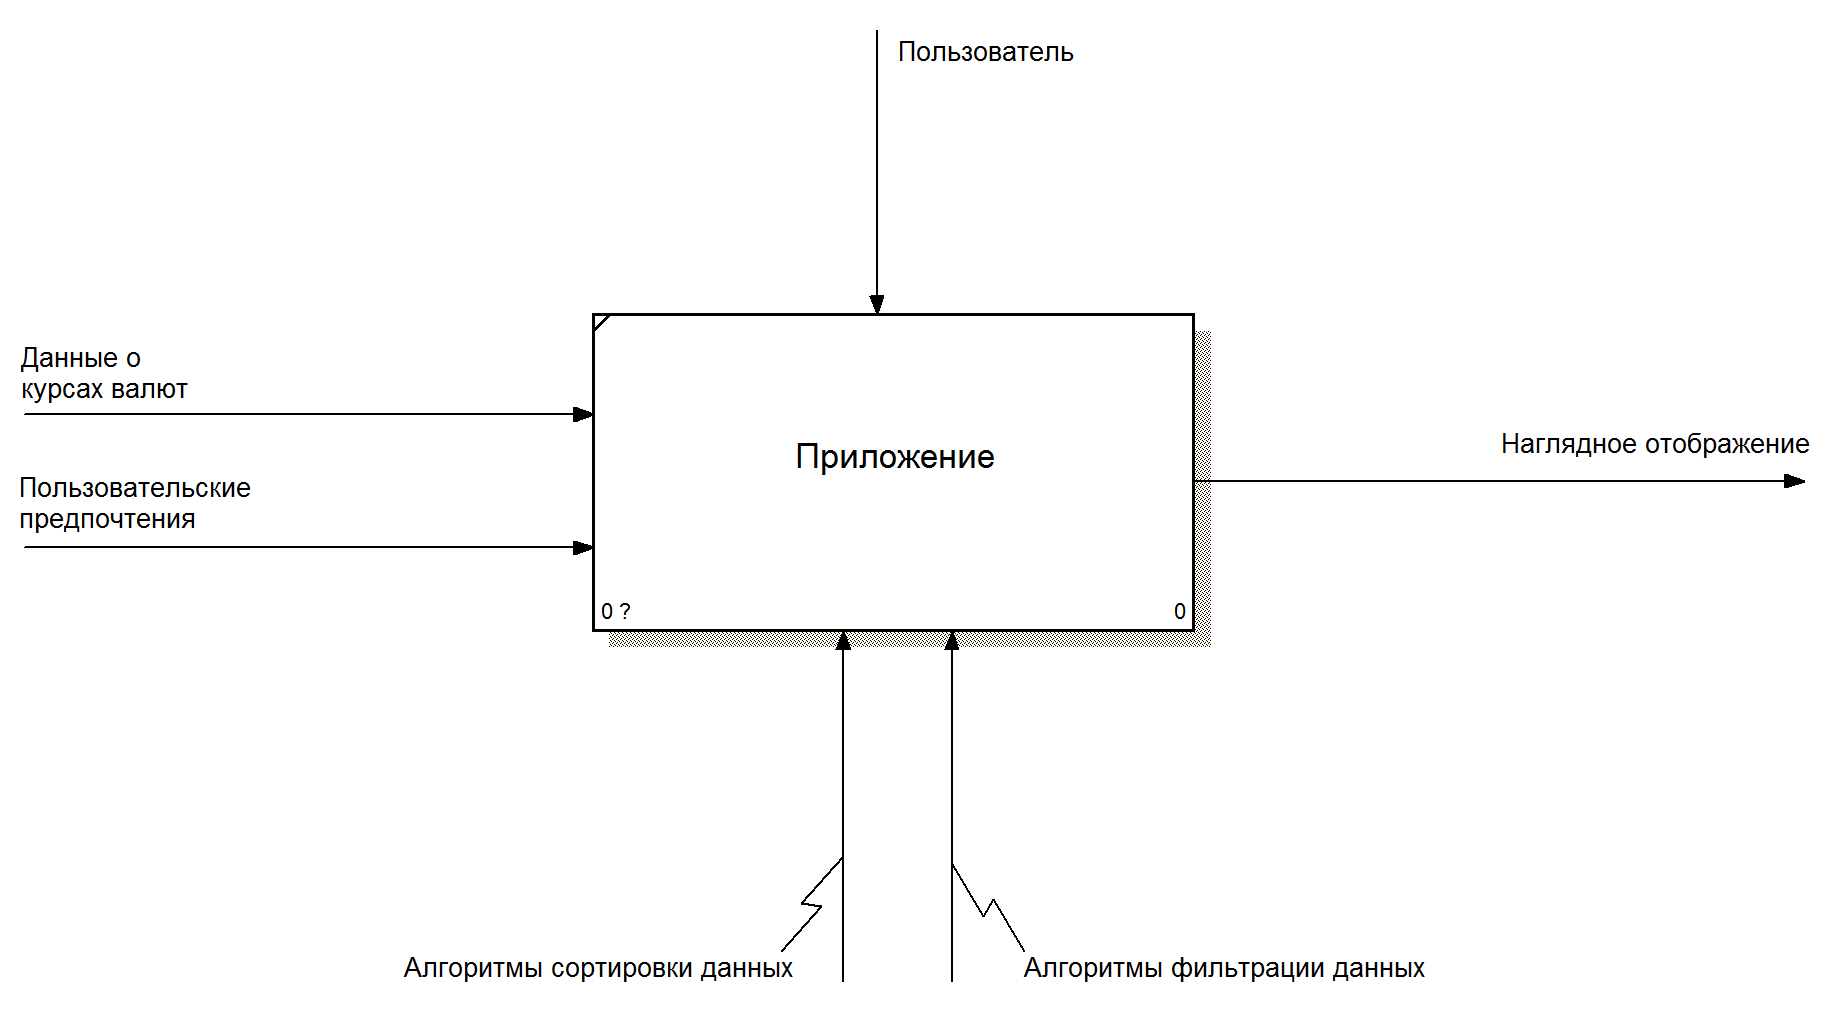
\includegraphics[width=150mm]{pic/IDEF0}
  \caption{Диаграмма декомпозиции \\ верхнего уровня}
  \label{fig:idef0}
\end{figure}

Из этой диаграммы видно, что входом системы служат данные о курсах валют,
а также личные предпочтения пользователя,
результатом работы системы являются финансовые данные,
прошедшие этапы сортировки, и фильтрации по определенным правилам,
управление осуществляет пользователь приложения.


\pagebreak
% application
На рисунке~\ref{fig:idef0_app} представлена диаграмма декомпозиции
приложения.

\begin{figure}[h!]
  \centering
  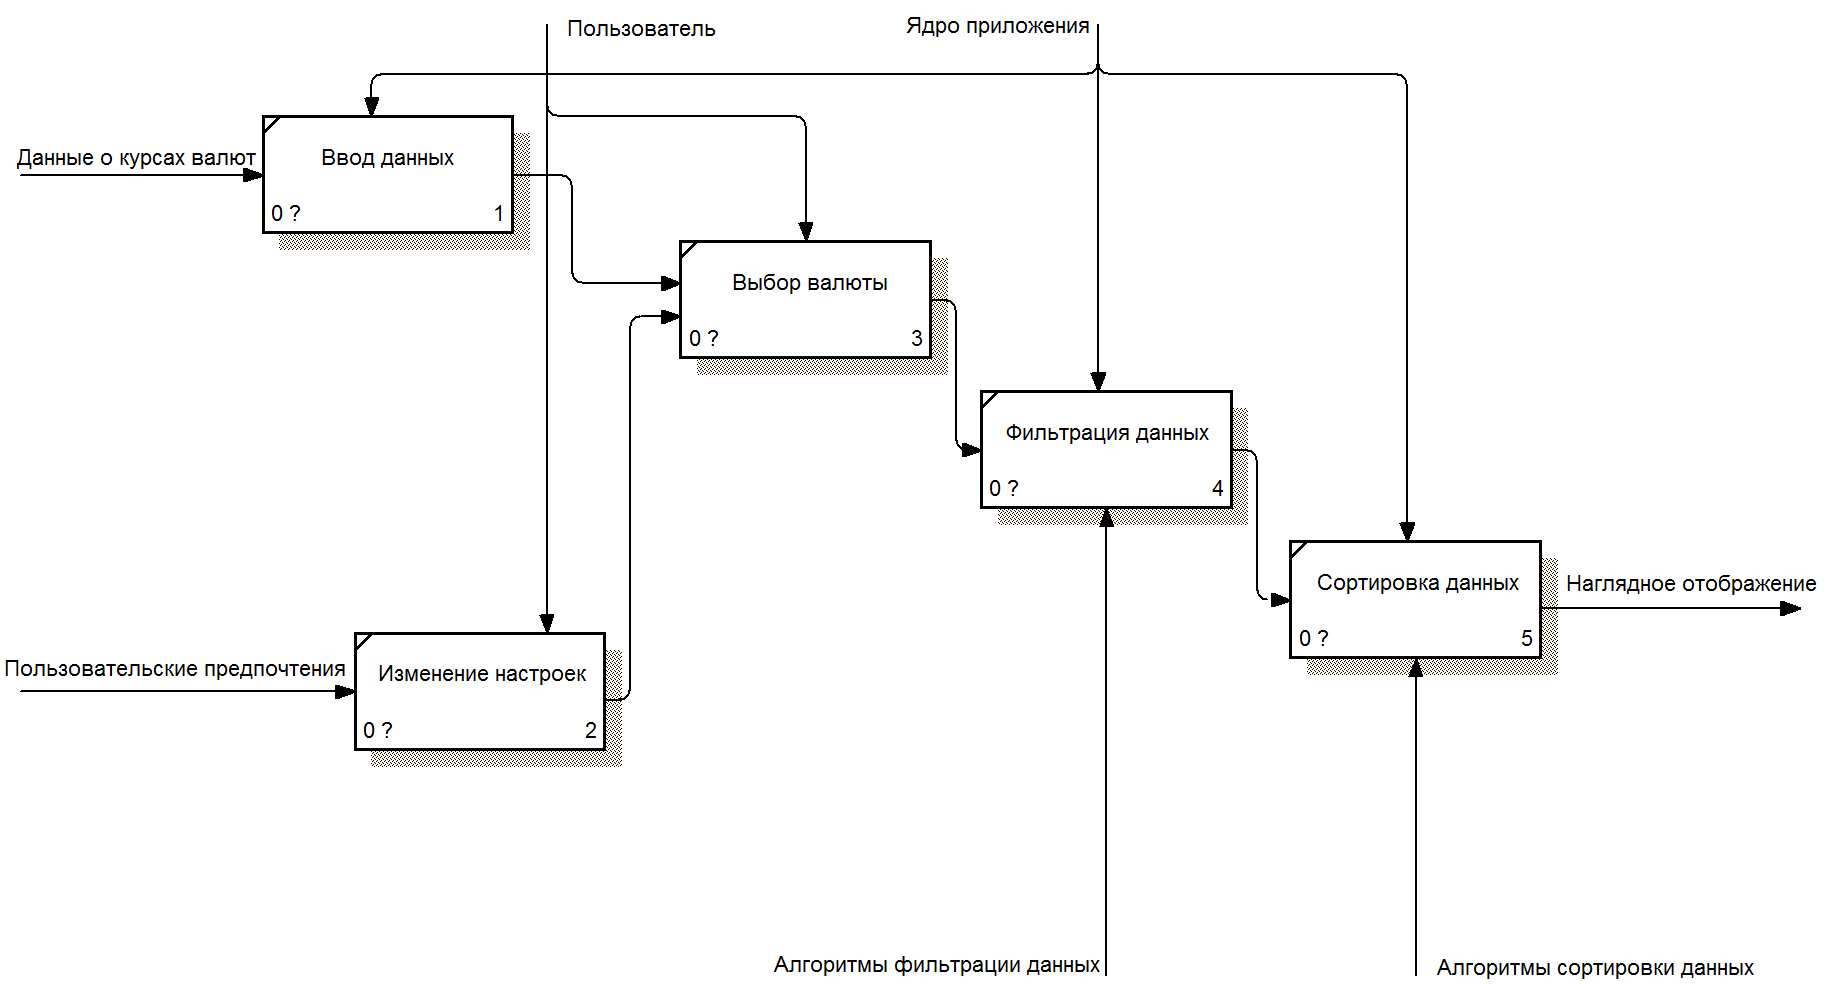
\includegraphics[width=150mm]{pic/IDEF0_decomposition}
  \caption{Диаграмма декомпозиции приложения}
  \label{fig:idef0_app}
\end{figure}

В соответствии с диаграммой, работу приложения можно разделить
на следующие части:
\begin{itemize}
  \item ввод данных;
  \item изменение настроек приложения;
  \item выбор валют;
  \item фильтрацая данных;
  \item сортировка данных.
\end{itemize}

Входом для блока <<Изменение настроек>> являются пользовательские
предпочтения, а выходом --- набор настроек, сохраненных в системе.

Финансовые данные, поступаемые на вход в блок <<Ввод данных>>
преобразуются в модели данных и созраняются в системе
для дальнейшего использования.

Выбор валюты производится на основании поступивших данных,
преобразуются в структурированную финансовую информацию.

Фильтрация данных представляет собой процесс отсеивания нулевых
значений, а также отбор данных по конкретной категории (валюте). 

Сортировку требуется производить для наглядного отображения курсов
валют в списке, по типу <<от наилучшего к наихудшему>>.


\pagebreak
% settings
Рассмотрим более подробно схему выбора настроек приложения,
представленную на рисунке~\ref{fig:idef3_settings}.

\begin{figure}[h!]
  \centering
  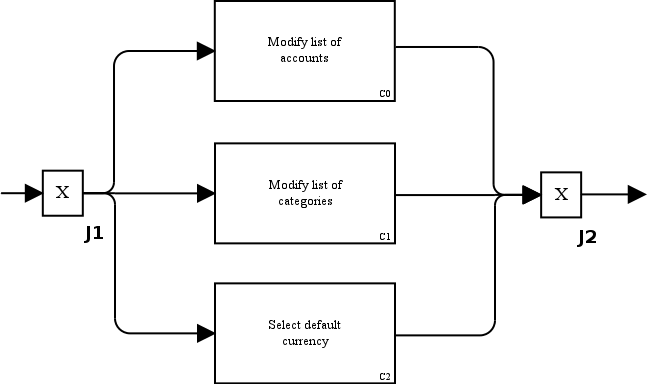
\includegraphics[width=150mm]{pic/idef3_settings}
  \caption{Диаграмма выбора настроек приложения}
  \label{fig:idef3_settings}
\end{figure}

В соответствии с диаграммой выбора настроек приложения,
пользователь имеет следующие возможности:
\begin{itemize}
  \item выбор города;
  \item просмотр истории версий приложения;
  \item просмотр общей информации о приложении с возможностью
    обратной связи с разработчиком приложения.
\end{itemize}

Выбор города может завершиться как сохранением изменений,
так и без. Как только пользователь изменяет выбранный город,
новые данные скачиваются в автоматическом режиме,
фильтруются, сортируются и отображаются пользователю в
виде упорядоченного списка.


\pagebreak
% input
Рассмотрим диаграмму процесса ввода данных,
представленную на рисунке~\ref{fig:idef3_input}.

\begin{figure}[h!]
  \centering
  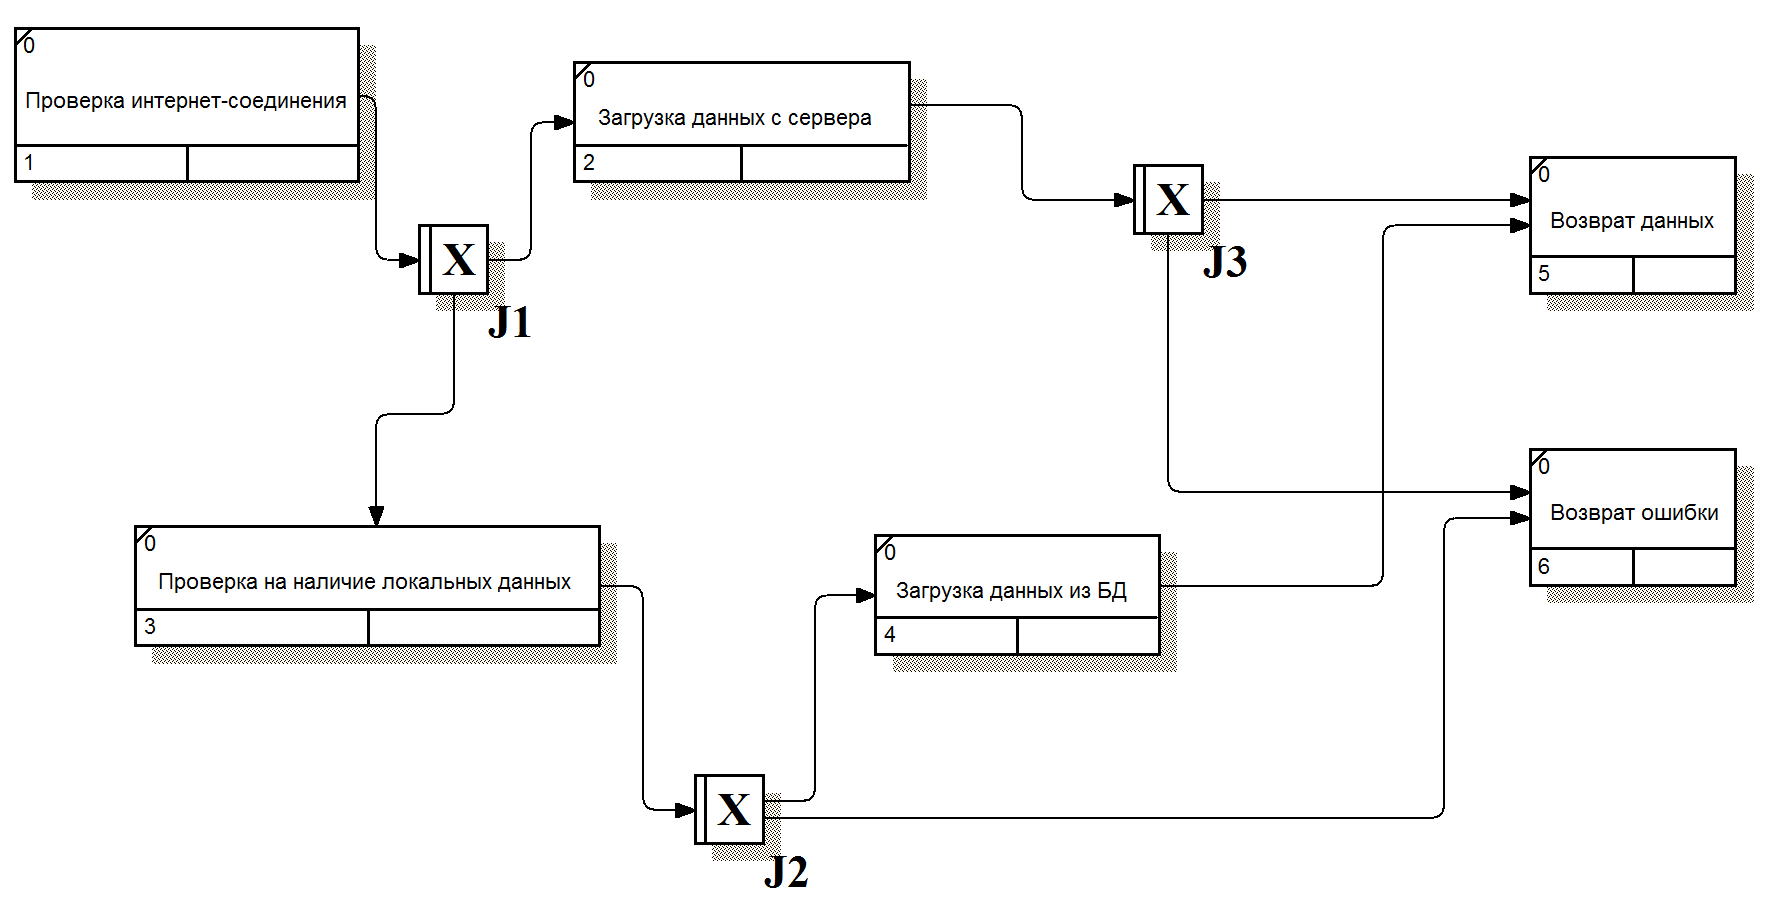
\includegraphics[width=150mm]{pic/IDEF3_load_data}
  \caption{Диаграмма процесса ввода данных}
  \label{fig:idef3_input}
\end{figure}

В соответствии с диаграммой процесса ввода данных, в первую очередь
происходит проверка на наличие интернет-соединения, тем самым
определяется источник данных --- сервер, или же локальное
хранилище данных.
В зависимости от результатов, пользователю
будет отображена различная информация: информация о курсах валют,
или же ошибка интернет-соединения.


% \pagebreak
% input
Далее рассмотрим процесс сортировки данных,
представленный на рисунке~\ref{fig:idef3_sort}.

\begin{figure}[h!]
  \centering
  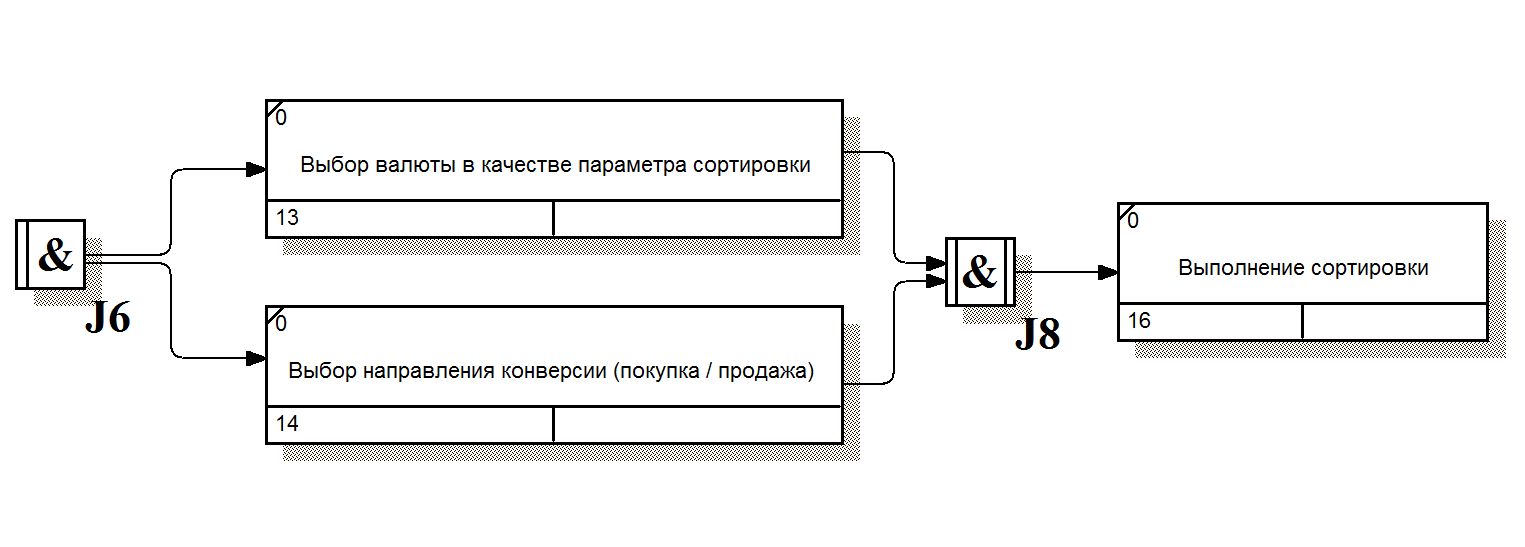
\includegraphics[width=150mm]{pic/IDEF3_sort}
  \caption{Диаграмма процесса сортировки данных}
  \label{fig:idef3_sort}
\end{figure}

\pagebreak

В соответствии с представленной на рисунке~\ref{fig:idef3_sort} диаграммой,
процесс сортировки данных предполагает некоторые параметры:
\begin{itemize}
  \item выбор валюты (доллар США, евро, российский рубль и др.);
  \item выбор направления конверсии (покупка или продажа валюты).
\end{itemize}

Начальные значения этих параметров задаются системой: валюта --- доллар США,
направление конверсии --- продажа валюты банком.

Пользователь имеет возможность изменить эти параметры,
перейдя на другой экран (экран <<Евро>>, <<Рос. рубль>> и др.),
или коснувшись кнопок <<Банк покупает>>, <<Банк продаёт>>.


\subsection{Пользовательский интерфейс системы}

В данном разделе будет рассмотрен дизайн интерфейса системы с точки зрения
конечного пользователя.

Приложения, разрабатываемые для мобильных платформ, можно разделить
на экраны --- различные части приложения, выполняющие предопределенную роль.

Примерами таких экранов для разрабатываемого приложения являются:
\begin{itemize}
  \item главный экран;
  \item экран просмотра детальной информации об отделении;
  \item экран поиска;
  \item экран изменения настроек;
  \item экран конвертера валют.
\end{itemize}

Главный экран приложения отображает информацию о наилучшем курсе в момент
использования приложения, список отделений с указанием их названия,
местоположения и курса продажи банком доллара США.

\pagebreak


На рисунке~\ref{fig:screen_main} представлен скриншот главного экрана приложения.

\begin{figure}[h!]
  \centering
  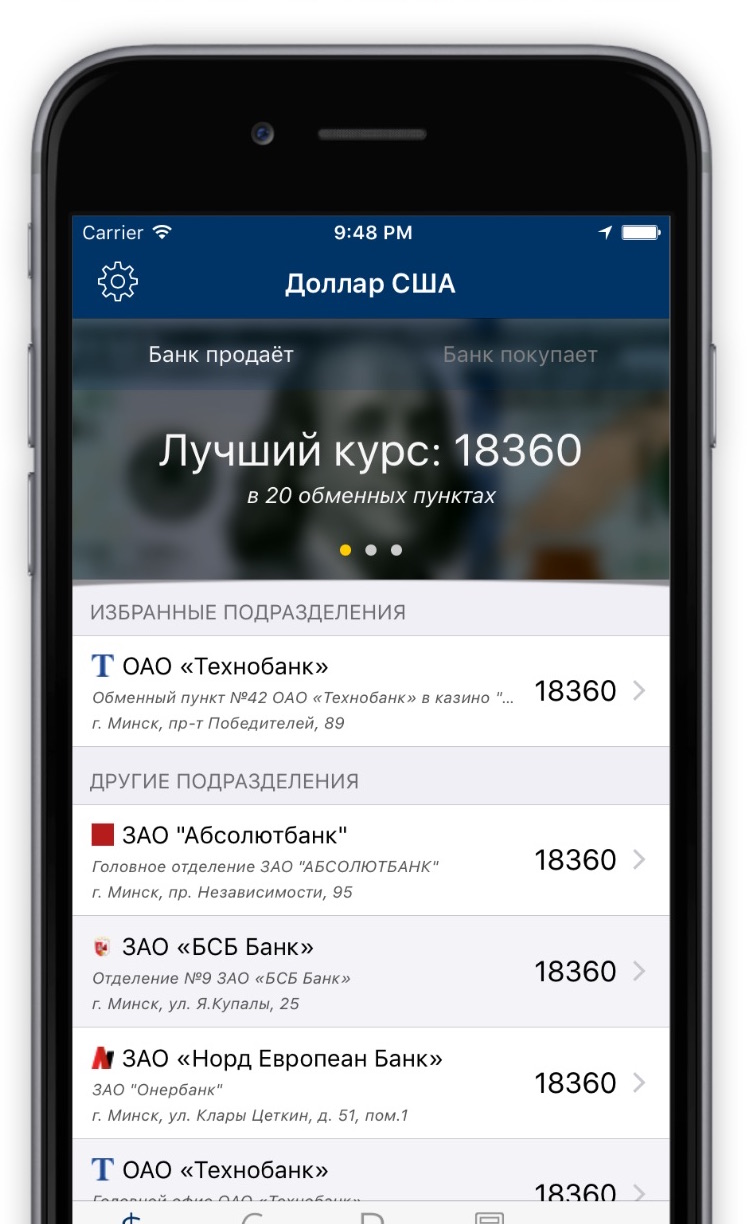
\includegraphics[width=80mm]{pic/screen_main}
  \caption{Главный экран приложения}
  \label{fig:screen_main}
\end{figure}

По нажатию на иконку настроек (левый верхний угол скриншота)
происходит переход к настройкам приложения. Верхняя область
приложения представляет собой представление (англ. view),
с возможность перелистывания. Кроме отображения информации
о лучшем курсе можно также просмотреть информацию о среднем
курсе и курсе Национального банка Республики Беларусь. 

По нажатию на элемент списка с отделениями отображается
экран с детальной информацией об отделении.

Пользователь имеет возможность изменить направление
конверсии приложения. По нажатию на элемент <<Банк покупает>>
выполнится упорядочивание данных. 

\pagebreak

На рисунке~\ref{fig:screen_details} представлен скриншот экрана, отображающего
детальную информацию об отделении.

\begin{figure}[h!]
  \centering
  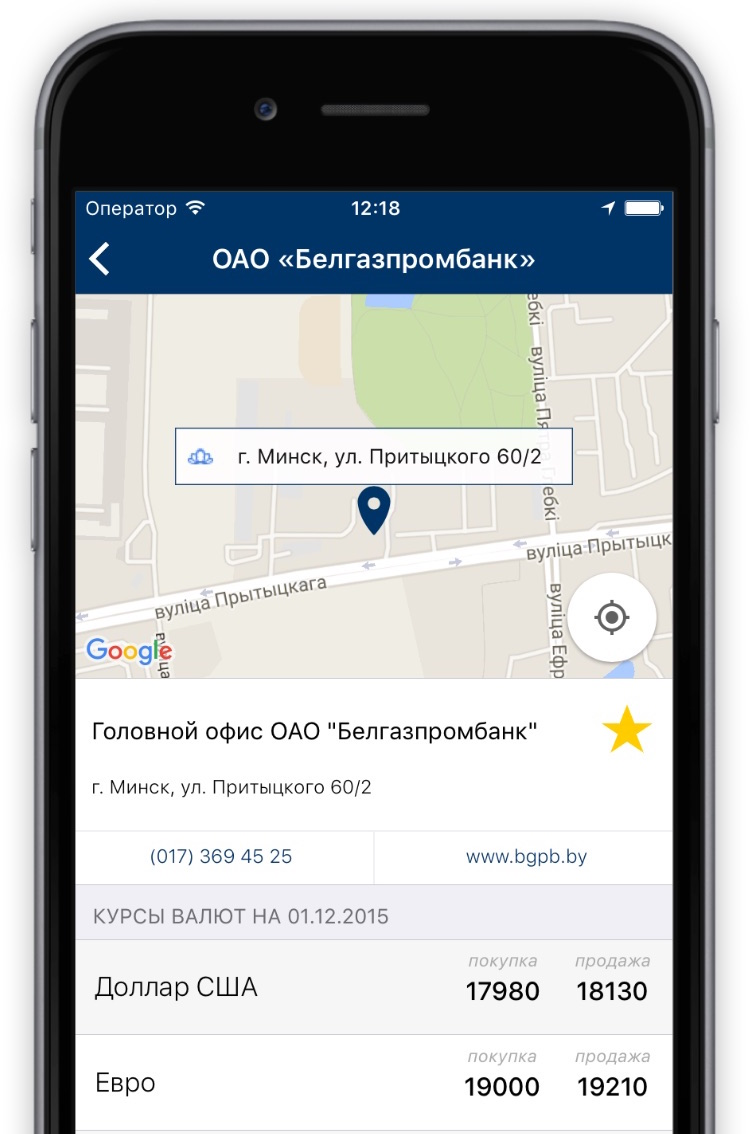
\includegraphics[width=90mm]{pic/screen_details}
  \caption{Экран детальной информации об отделении}
  \label{fig:screen_details}
\end{figure}

Пользователь имеет возможность изменять детализацию карты,
добавлять отделение в категорию <<Избранные>>, совершать
звонок, а также переходить на сайт банка. В нижей части
экрана отображаются доступные валюты этого отделения,
указана дата обновления информации. 


\pagebreak
На рисунке~\ref{fig:screen_converter} представлен скриншот
экрана конвертера валют.

\begin{figure}[h!]
  \centering
  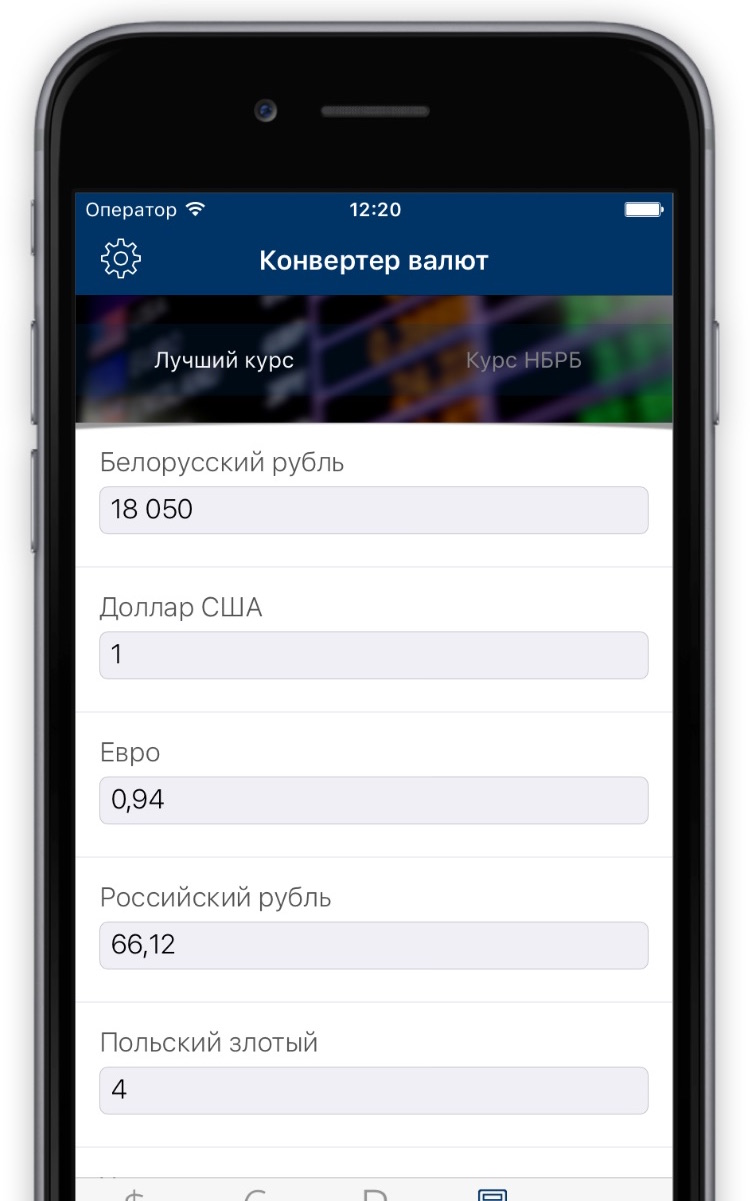
\includegraphics[width=90mm]{pic/screen_converter}
  \caption{Экран конвертера валют}
  \label{fig:screen_converter}
\end{figure}

Пользователь вводит значение в ячейке любой валюты, все
остальные значения рассчитываются автоматически и заполняют
пустые ячейки.

В качестве значений для расчёта используются либо критические
значения по каждой из валют (лучшие значения курсов), либо
курсы валют Национального банка Республики Беларусь. Выбор
производит пользователь.


\pagebreak
На рисунке~\ref{fig:screen_settings} представлен скриншот экрана
настроек приложения.

\begin{figure}[h!]
  \centering
  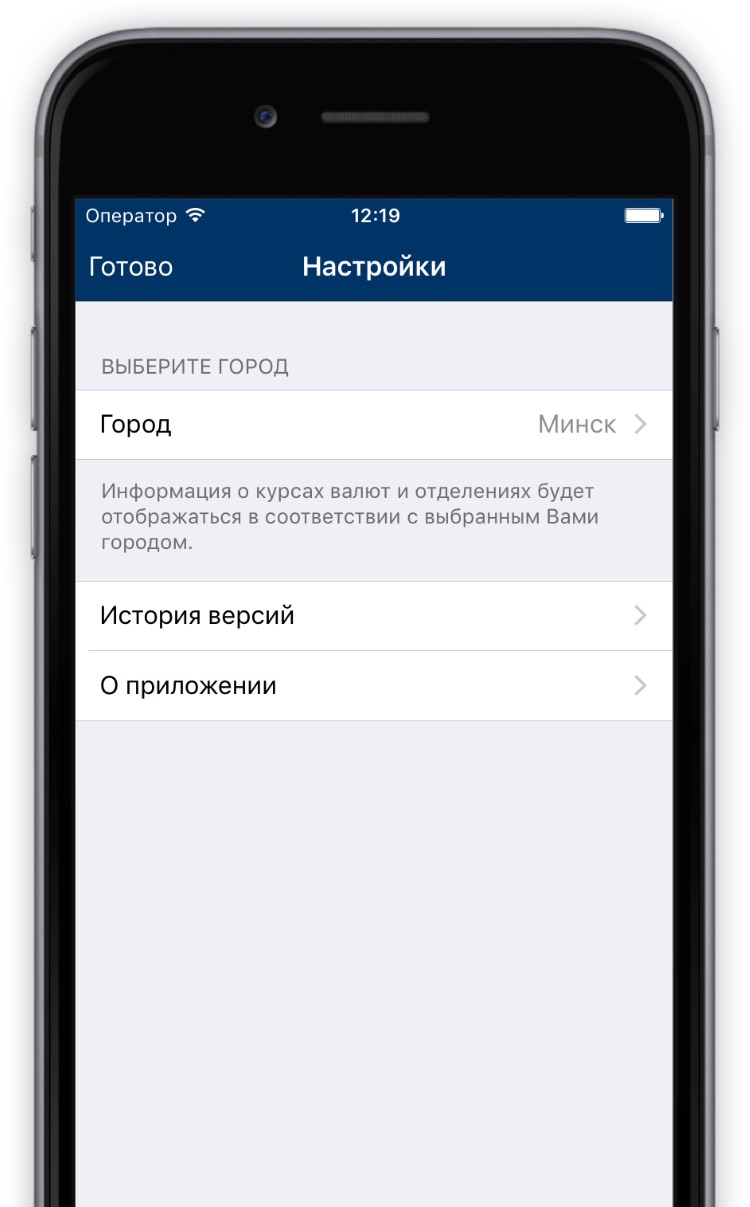
\includegraphics[width=90mm]{pic/screen_settings}
  \caption{Экран настроек приложения}
  \label{fig:screen_settings}
\end{figure}

Экран настроек приложения открывается путем
нажатия на кнопку, расположенную в левом верхнем
углу каждого экрана приложения.
Находясь на этом экране, пользователь может изменить
город, для которого будет отображаться список отделений,
просмотреть историю версий приложений, общую информацию
о приложении, а также связаться с разработчиком приложения.
